\documentclass{article}
\usepackage{tikz}
\usetikzlibrary{calc}
\usepackage{relsize}

\tikzset{fontscale/.style = {font=\relsize{#1}}
    }

\begin{document}
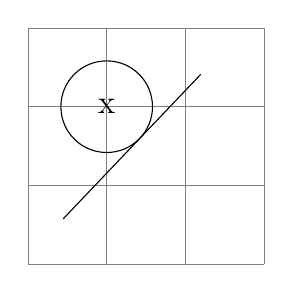
\begin{tikzpicture}
  \draw [help lines] (0,0) grid (3,3);
  \coordinate (a) at (rnd,rnd);
  \coordinate (b) at (3-rnd,3-rnd);
  \draw (a) -- (b);
  \node (c) at (1,2) [fontscale=1] {x};
  \draw let \p1 = ($ (a)!(c)!(b) - (c) $),
            \n1 = {veclen(\x1,\y1)}
        in circle [at=(c), radius=\n1];
\end{tikzpicture}
\end{document}
